\documentclass[11pt, oneside]{article} 
\usepackage{geometry}
\geometry{letterpaper} 
\usepackage{graphicx}
	
\usepackage{amssymb}
\usepackage{amsmath}
\usepackage{parskip}
\usepackage{color}
\usepackage{hyperref}

\graphicspath{{/Users/telliott/Github/figures/}}
% \begin{center} \includegraphics [scale=0.4] {gauss3.png} \end{center}

\title{Introduction}
\date{}

\begin{document}
\maketitle
\Large

This book has been modified from a previous project, where it comprised the first several chapters of another project titled \emph{Best of Calculus}.  That book is here:

\url{https://github.com/telliott99/calculus_book}

I decided to make these chapters separate because the overall size of the big book makes it hard to focus on the Precalculus topics.  These chapters have been the recipient of much recent attention on my part.

I wrote much of this originally as short explanations for my son Sean as he studied calculus in high school.  It bothers me that so often the good stuff gets left out at that level. 

\begin{center} 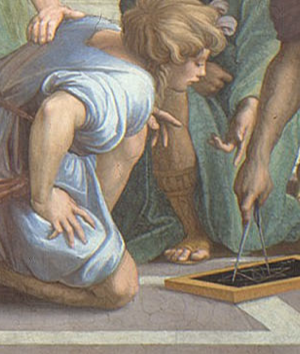
\includegraphics [scale=0.4] {school_of_athens.png} \end{center}

(The image is a detail from a painting entitled "School of Athens", and it was used as the front cover of a wonderful book annotating the Heath translation of Euclid's \emph{Elements}).

It took a genius to figure it out the first time, but it is within anyone's grasp to appreciate what they found.  I imagine myself looking over Archimedes' shoulder as he explains it to me.

There is a lot of geometry here.  Most scientists I've met loved geometry in school.  Proof is central to the enterprise. One of the most interesting features of this book is the natural use of proofs that I have tried to make as simple and easy to follow as possible.

My favorite authors on calculus including precalculus are Morris Kline, Richard Hamming, and Gil Strang.  I highly recommend Simmons, if you can find a copy.

Finally, a saying attributed to Manaechmus (speaking to Alexander the Great), "there is no royal road to geometry".  Which means, practically, learning mathematics requires that you follow the argument with pencil and paper and work out each step yourself, to your own satisfaction.  That is the only way of really learning, and at heart, one of the reasons I wrote this book.

I express my sincere thanks to the authors of my favorite books, which are listed in the references and mentioned at various places in the text.  Almost everything in here was appropriated from them, and styled to my taste.  I offer my profound thanks also to Eugene Colosimo, S.J.  He was, for me, the best of a bunch of very special teachers.

If I stole your figure off the internet, I'm sorry.  I intended to redraw it but have not yet found the time.  

We start with my favorite mathematician, Archimedes.

You can find the current version of this book on github here:

\url{https://github.com/telliott99/precalculus}

\end{document}